\documentclass[authoryear,preprint]{sigplanconf}
\usepackage{amsmath}
\usepackage{listings} 
\usepackage{stmaryrd}
\usepackage{latexsym}
\usepackage{amssymb}
\usepackage{xcolor}
\usepackage{courier}
\usepackage{thmtools}
\usepackage{bbold}
\usepackage{tikz}

\newcommand{\lolli}{\multimap} 
\newcommand{\cubt}{\mathbb{T}}
\newcommand{\nodet}[2]{\fcolorbox{black}{white}{$#1$}\fcolorbox{black}{gray!20}{$#2$}}

\begin{document}
\special{papersize=8.5in,11in}
\setlength{\pdfpageheight}{\paperheight}
\setlength{\pdfpagewidth}{\paperwidth}

\newcommand{\alt}{~|~}
\lstnewenvironment{code}{\lstset{basicstyle={\sffamily\footnotesize}}}{}

\lstset{frame=none,
         language=Haskell,
         basicstyle=\sffamily, 
         numberstyle=\tiny,
         numbersep=5pt,
         tabsize=2,    
         extendedchars=true,
         breaklines=true,   
         breakautoindent=true,
         keywordstyle=\color{black},
         captionpos=b,
         stringstyle=\color{black}\ttfamily,
         showspaces=false,  
         showtabs=false,    
         framexleftmargin=2em,
         framexbottommargin=1ex,
         showstringspaces=false
         basicstyle=\sffamily,
         columns=[l]flexible,
         flexiblecolumns=true,
         aboveskip=\smallskipamount,
         belowskip=\smallskipamount,
         lineskip=-1pt,
         xleftmargin=1em,
         escapeinside={/+}{+/},
         keywords=[1]{Monad,Just,Nothing,type,data,right,left,id,where,do,
                     if,then,else,let,in},
         literate=
           {+}{{$\;+\;$}}1 
           {/}{{$/$}}1 
           {*}{{$\;*\;$}}1
           {=}{{$=\ $}}1 
           {/=}{{$\not=$}}1
           {[]}{$[\;]$}2
           {<}{{$<$}}1 
           {>}{{$>$}}1 
           {++}{{$+\!\!\!+\;$}}1 
           {::}{{$:\mkern -2.5mu:\;$}}1
           {&&}{{$\&\!\!\!\&$}}2
           {:=:}{{$:\mkern -2mu=\mkern -2mu:\;$}}3
           {:+:}{{$:\mkern -5mu+\mkern -5mu:\;$}}3
           {:-:}{{$:\mkern -5mu-\mkern -5mu:\;$}}3
           {:*:}{{$:\mkern -5mu*\mkern -5mu:\;$}}3
           {$}{{\texttt{\$}\hspace{0.5em}}}1
           {`}{$^\backprime$}1
           {==}{{$=\!=\;$}}2
           {===}{{$\equiv\;$}}2
           {->}{{$\rightarrow\;$}}2 
           {>=}{{$\geq$}}2 
           {<=}{{$\leq$}}2 
           {>=0}{{$\geq_\zerog\;$}}2 
           {<=0}{{$\leq_\zerog\;$}}2 
           {==0}{{$=_\zerog\;$}}2 
           {>0}{{$>_\zerog\;$}}2 
           {<0}{{$<_\zerog\;$}}2 
           {<-}{{$\leftarrow$}}2
           {=>}{{$\Rightarrow\;$}}2
           {<<}{{$\ll$}}2 
           {>>}{{$\gg\;$}}2
           {>>>}{{$\ggg\;$}}3 
           {<<<}{{$\lll\;$}}3
           {>>=}{{$\gg\mkern -2.5mu=\;$}}3
           {=<<}{{$=\mkern -2.5mu\ll\;$}}3
           {<|}{$\lhd\;$}2
           {<||}{$\unlhd\;$}2
           {\ ||\ }{$\|$}1
           {\\}{$\lambda$}1
           {:>}{{$\rhd$}}2
           {||>}{{$\unrhd$}}2
           {_}{{$\_$}}1
           {_B}{{$_b$}}2
           {forall}{{$\forall$}}1
}

\lstset{postbreak=\raisebox{0ex}[0ex][0ex]
        {\ensuremath{\hookrightarrow}}}
\lstset{breaklines=true, breakatwhitespace=true}
\lstset{numbers=none, numbersep=5pt, stepnumber=2, numberstyle=\scriptsize}
\lstset{rangeprefix=/*!\ , rangesuffix=\ !*\/, includerangemarker=false}

%% double-blind reviewing...
\title{Cubical Types with Positive and Negative Polarities}
\authorinfo{}{}{}
\maketitle

\begin{abstract}
\ldots
\end{abstract}

%%%%%%%%%%%%%%%%%%%%%%%%%%%%%%%%%%%%%%%%%%%%%%%%%%%%%%%%%%%%%%%%%%%%%%%%%%%%%%
\section{Introduction}

The \textbf{Int} construction or the $\mathcal{G}$ construction are neat. As
Neel K. explains, given first-order types and feedback you get higher-order
functions. But if you do the construction on the additive structure, you lose
the multiplicative structure. It turns out that this is related to a deep
open problem in algebraic topology and homotopy theory that was recently
solved. We ``translate'' that solution to a computational type-theoretic
world. This has evident connections to homotopy (type?) theory that remain to
be investigated.

%%%%%%%%%%%%%%%%%%%%%%%%%%%%%%%%%%%%%%%%%%%%%%%%%%%%%%%%%%%%%%%%%%%%%%%%%%%%%%
\section{The \textbf{Int} Construction} 

Explain in detail perhaps with Haskell embedding and type functions etc. The
key insight it to add ``negative'' types representing demand for values. This
is how you get functions.

%%%%%%%%%%%%%%%%%%%%%%%%%%%%%%%%%%%%%%%%%%%%%%%%%%%%%%%%%%%%%%%%%%%%%%%%%%%%%%
\section{The Problem and the Intuitive Solution}

We lose the multiplicative structure. No evident way to define the
multiplication functor. Perhaps there is a clever way. But this turns out to
be a well-known open problem. Review the problem and tell the story from the
algebraic topology perspective.

Regular first-order types are viewed as 1-dimensional cubes. Generalize to
$n$-dimensional cubes. 

%%%%%%%%%%%%%%%%%%%%%%%%%%%%%%%%%%%%%%%%%%%%%%%%%%%%%%%%%%%%%%%%%%%%%%%%%%%%%%
\section{The Formal Construction} 

We use $\tau$ for regular first-order types which include the empty type, the
unit type, and conventional sum and product types.  We use $\cubt$ for
general $n$-dimensional cubical types. An $n$-dimensional cubical type
$\nodet{\cubt_1}{\cubt_2}$ consists of a positive subspace $\cubt_1$ and a
negative subspace $\cubt_2$ (shaded in gray). Each of the subspaces are
cubical types of a lower dimension; the 1-dimensional case reduces to plain
first-order types. As we explain below, cubical types are closed under sums,
differences, products, and can express higher-order functions $\cubt_1 \lolli
\cubt_2$ as $(\ominus \cubt_1) \oplus \cubt_2$. The syntax of the types is
summarized below:
\[\begin{array}{rcl}
\tau &::=& 0 \alt 1 \alt \tau_1 + \tau_2 \alt \tau_1 * \tau_2 \\
\\
\cubt &::=& \tau \alt \nodet{\cubt_1}{\cubt_2} 
      \alt \cubt \oplus \cubt 
      \alt \cubt \otimes \cubt 
      \alt \ominus \cubt 
\end{array}\]
Examples of 1-dimensional cubical types include all the regular first-order
types $\tau$. A 2-dimensional cubical type looks like
$\nodet{\tau_1}{\tau_2}$ which intuitively corresponds to the difference
$\tau_1 - \tau_2$ of the two types. A 3-dimensional cubical type looks like
$\nodet{(\nodet{\tau_1}{\tau_2})}{(\nodet{\tau_3}{\tau_4})}$ which
intuitively corresponds to the iterated difference of types
$(\tau_1-\tau_2)-(\tau_3-\tau_4)$ where the successive colors from the root
encode the sign as follows: white in the outermost box corresponds to a
positive polarity and gray in the outermost box corresponds to a negative
polarity; then, as we move inwards the polarities alternate for every change
of color. It is possible for cubical types not be balanced in general but it
is always possible to extend the shorter subtree to an arbitrary depth using
the fact (to be justified later) that~$\tau$ is equivalent to
$\nodet{\tau}{0}$.

We now explain how cubical types are closed under sum, difference, and
products. In the recursive definitions below, we assume that the types have
been extended to be balanced as needed:
\[\begin{array}{rcl}
\ominus~\tau &=& \tau \\
\ominus~\nodet{\cubt_1}{\cubt_2} &=& \nodet{\ominus~\cubt_2}{\ominus~\cubt_1} \\
\\
\tau_1 \oplus \tau_2 &=& \tau_1 + \tau_2 \\
(\nodet{\cubt_1}{\cubt_2}) \oplus (\nodet{\cubt_3}{\cubt_4}) &=& 
  \nodet{\cubt_1 \oplus \cubt_3}{\cubt_2 \oplus \cubt_4} \\
\\
\tau_1 \otimes \tau_2 &=& \tau_1 * \tau_2 \\
\tau \otimes (\nodet{\cubt_1}{\cubt_2}) &=& 
  \nodet{\tau \otimes \cubt_1}{\tau \otimes \cubt_2} \\
(\nodet{\cubt_1}{\cubt_2}) \otimes \cubt &=& 
  \nodet{\cubt_1 \otimes \cubt}{\cubt_2 \otimes \cubt}
\end{array}\]

\begin{figure*}
\[\begin{array}{c}
\nodet{\tau_1}{\tau_2}
\quad\otimes\quad
\nodet{(\nodet{\tau_3}{\tau_4})}{(\nodet{\tau_5}{\tau_6})} = 
\\
\nodet{(\nodet{{(\nodet{\tau_1*\tau_3}{\tau_1*\tau_4})}}
              {{(\nodet{\tau_1*\tau_5}{\tau_1*\tau_6})}})}
      {(\nodet{{(\nodet{\tau_2*\tau_3}{\tau_2*\tau_4})}}
              {{(\nodet{\tau_2*\tau_5}{\tau_2*\tau_6})}})}
\end{array}\]
\caption{\label{mult}Example of multiplication of two cubical types.}
\end{figure*}

A few examples might provide some needed intuition. First we note that the
general definitions of sum and product reduce to the conventional sums and
products for 1-dimensional types. Also the sum of 2-dimensional types reduces
to the sum used in the \textbf{Int} construction. The interesting new
development is the product definition. The example in Fig.~\ref{mult} shows
that in general the product of an $n$-dimensional type with an
$m$-dimensional type gives an $(n+m)$-dimensional type. For low dimensions
such as the ones used in the example above, it is possible to visualize what
is happening in coordinate space (see Fig.~\ref{multv}).

\begin{figure*}
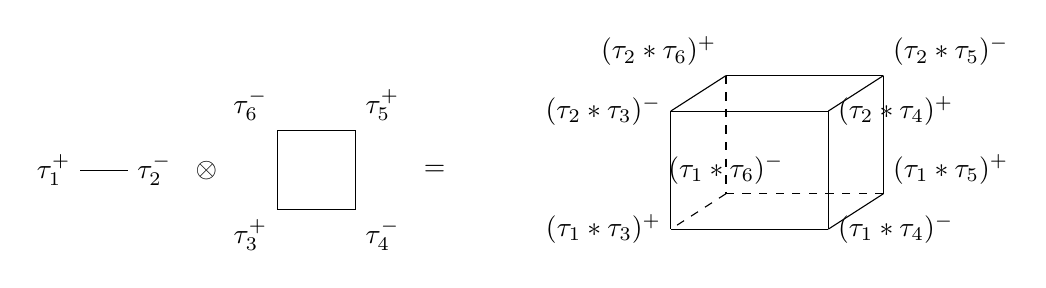
\begin{tikzpicture}
\node[left] at (0,0) {$\tau_1^+$};
\node[right] at (0.6,0) {$\tau_2^-$};
\draw[-] (0,0) -- (0.6,0);
\node at (1.6,0) {$\otimes$}; 
%%
\node[below left] at (2.5,-0.5) {$\tau_3^+$};
\node[below right] at (3.5,-0.5) {$\tau_4^-$};
\draw[-] (2.5,-0.5) -- (3.5,-0.5);
\draw[-] (2.5,-0.5) -- (2.5,0.5);
\node[above left] at (2.5,0.5) {$\tau_6^-$};
\node[above right] at (3.5,0.5) {$\tau_5^+$};
\draw[-] (2.5,0.5) -- (3.5,0.5);
\draw[-] (3.5,-0.5) -- (3.5,0.5);
%% 
\node at (4.5,0) {$=$};
%% 
\node[left] at (7.5,0.75) {$(\tau_2*\tau_3)^-$};
\node[right] at (9.5,0.75) {$(\tau_2*\tau_4)^+$};
\node[above right] at (10.2,1.2) {$(\tau_2*\tau_5)^-$};
\node[above left] at (8.2,1.2) {$(\tau_2*\tau_6)^+$};
%%
\node[left] at (7.5,-0.75) {$(\tau_1*\tau_3)^+$};
\node[right] at (9.5,-0.75) {$(\tau_1*\tau_4)^-$};
\node[above right] at (10.2,-0.3) {$(\tau_1*\tau_5)^+$};
\node[above] at (8.2,-0.3) {$(\tau_1*\tau_6)^-$};
%%
\draw[-] (7.5,0.75) -- (9.5,0.75);
\draw[-] (9.5,0.75) -- (10.2,1.2);
\draw[-] (10.2,1.2) -- (8.2,1.2);
\draw[-] (8.2,1.2) -- (7.5,0.75);
%%
\draw[-] (7.5,-0.75) -- (9.5,-0.75);
\draw[-] (9.5,-0.75) -- (10.2,-0.3);
\draw[-,dashed] (10.2,-0.3) -- (8.2,-0.3);
\draw[-,dashed] (8.2,-0.3) -- (7.5,-0.75);
%%
\draw[-] (7.5,0.75) -- (7.5,-0.75);
\draw[-] (9.5,0.75) -- (9.5,-0.75);
\draw[-] (10.2,1.2) -- (10.2,-0.3);
\draw[-,dashed] (8.2,1.2) -- (8.2,-0.3);
\end{tikzpicture}
\caption{\label{multv}Visualization of multiplication of two cubical types.}
\end{figure*}

\begin{verbatim}
There are zero objects of all depths:
  0, (0-0), (0-0)-0, ...
There are 1 objects of all depths:
  1, (1-0), (1-0)-0, ...

To complete the story we need to 
define morphisms. (More on this below.)
Once we have a notion of morphism we 
can check whether X + 0 is the same
as X etc. i.e., we can check all the 
ring equivalences. 

Ok so what are the morphisms between 
these cubical objects? We know what
they are for 1-dimensional cubes: 
they are the pi combinabors. We also
know what they are for the 2-dimensional 
cubes: a maps (A-B) ==> (C-D) 
is a Pi map between A+D <=> C+B. 
How to generalize this? 

Why is there no trace in the ring 
completion paper??? What are 
the morphisms in that paper?
\end{verbatim}

%%%%%%%%%%%%%%%%%%%%%%%%%%%%%%%%%%%%%%%%%%%%%%%%%%%%%%%%%%%%%%%%%%%%%%%%%%%%%%
\section{A Reversible Language with Cubical Types} 

Pi with cubical types

%%%%%%%%%%%%%%%%%%%%%%%%%%%%%%%%%%%%%%%%%%%%%%%%%%%%%%%%%%%%%%%%%%%%%%%%%%%%%%
\section{Related Work and Context}

A ton of stuff here. 

%%%%%%%%%%%%%%%%%%%%%%%%%%%%%%%%%%%%%%%%%%%%%%%%%%%%%%%%%%%%%%%%%%%%%%%%%%%%%%
\section{Conclusion}

%%%%%%%%%%%%%%%%%%%%%%%%%%%%%%%%%%%%%%%%%%%%%%%%%%%%%%%%%%%%%%%%%%%%%%%%%%%%%%
\bibliographystyle{abbrvnat}
\softraggedright
\bibliography{cites}

\end{document}



